\section{Introduction to digital signals}

\subsection*{Resources}

The following pages are based on slides developed by Prof. Maraso Yamashiro for the 2015 class on Fourier Analysis. Please work through the slides on the following pages and view the video afterwards.

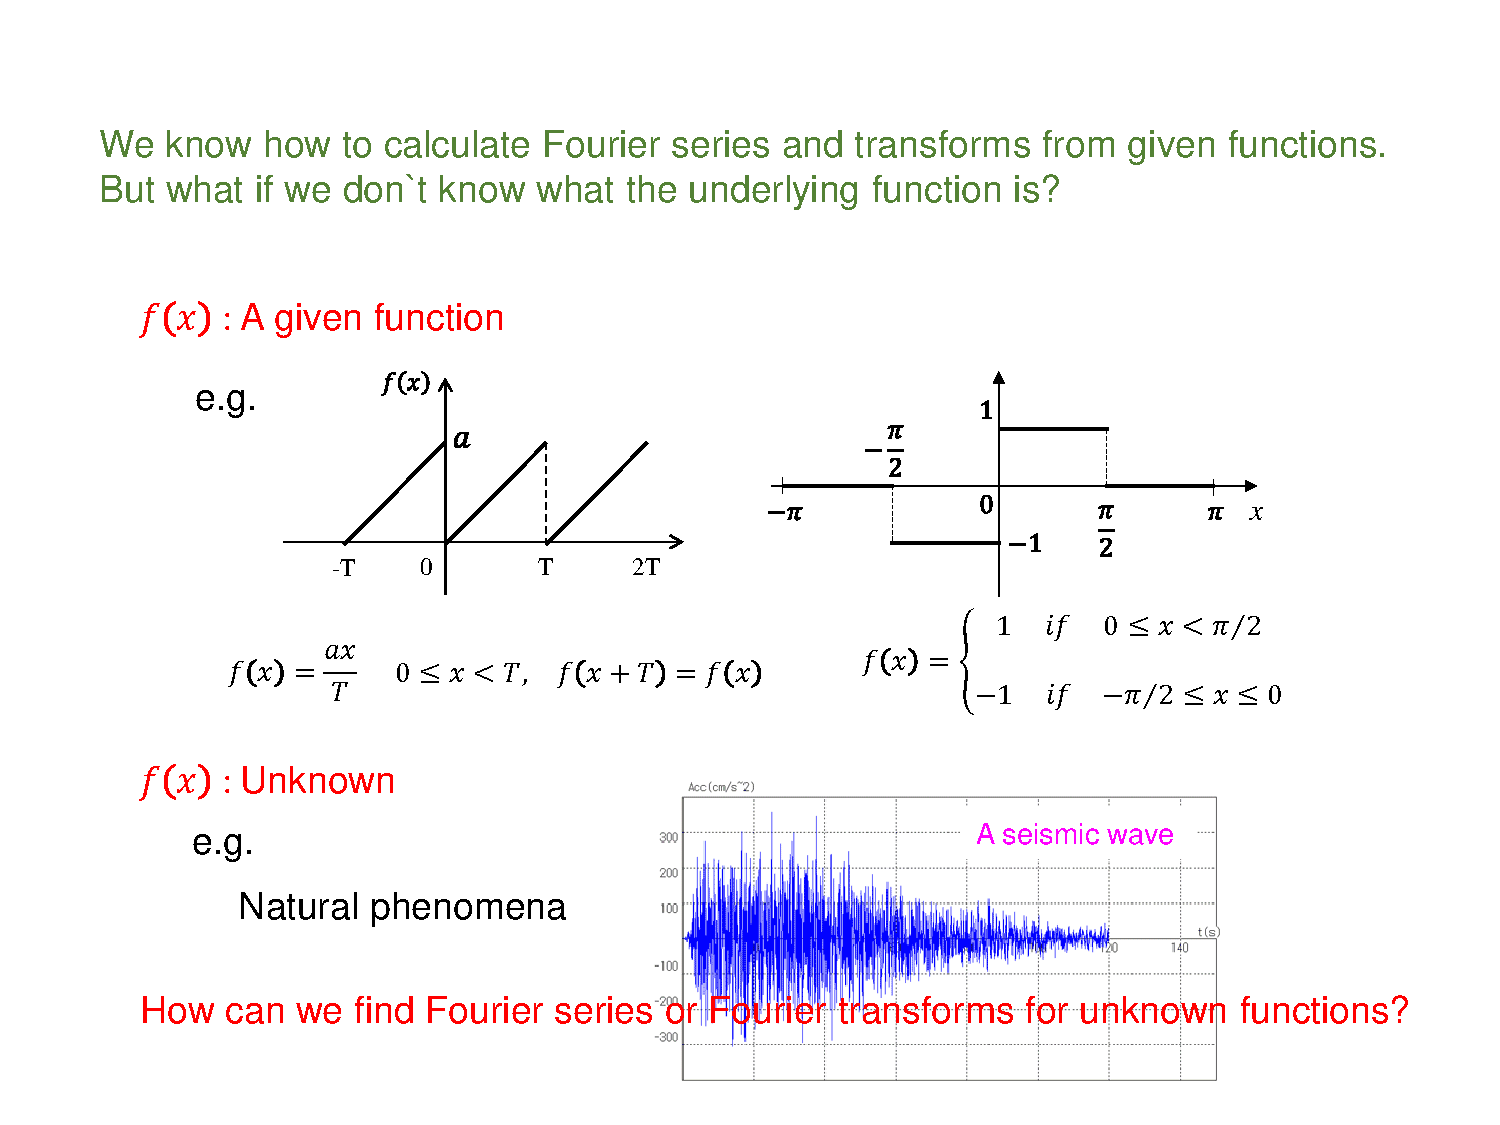
\includepdf[pages=-,pagecommand={},width=\textwidth,nup=1x2,frame=true]{discrete_1-5.pdf}

\begin{itemize}
    \item Video: \url{https://www.youtube.com/watch?v=yWqrx08UeUs&feature=youtu.be&t=47s}
\end{itemize}

\subsection*{Challenge}
1. An audio CD has a 44.1 kHz sampling rate. What is the highest frequency that experiences aliasing?

2. Write a sentence or two summarising what aliasing is and the Nyquist sampling theorem.

\subsection*{Solutions}
1. Write your solution X to 2 decimal places in units of kHz: \hash{xxx}{8a6fe0}

2. Check your answer with your partner and discuss any differences. Ask the teacher if you are unsure.

% Add something on quantisation?




%%%%%%%%%%%%%%%%%%%%%%%%%%%%%%%%%
\newpage
%%%%%%%%%%%%%%%%%%%%%%%%%%%%%%%%%
\section{Discrete Fourier Transform: Coefficients}

\subsection*{Resources}

The following pages are based on slides developed by Prof. Maraso Yamashiro for the 2015 class on Fourier Analysis. Please follow the derivation on the following pages.

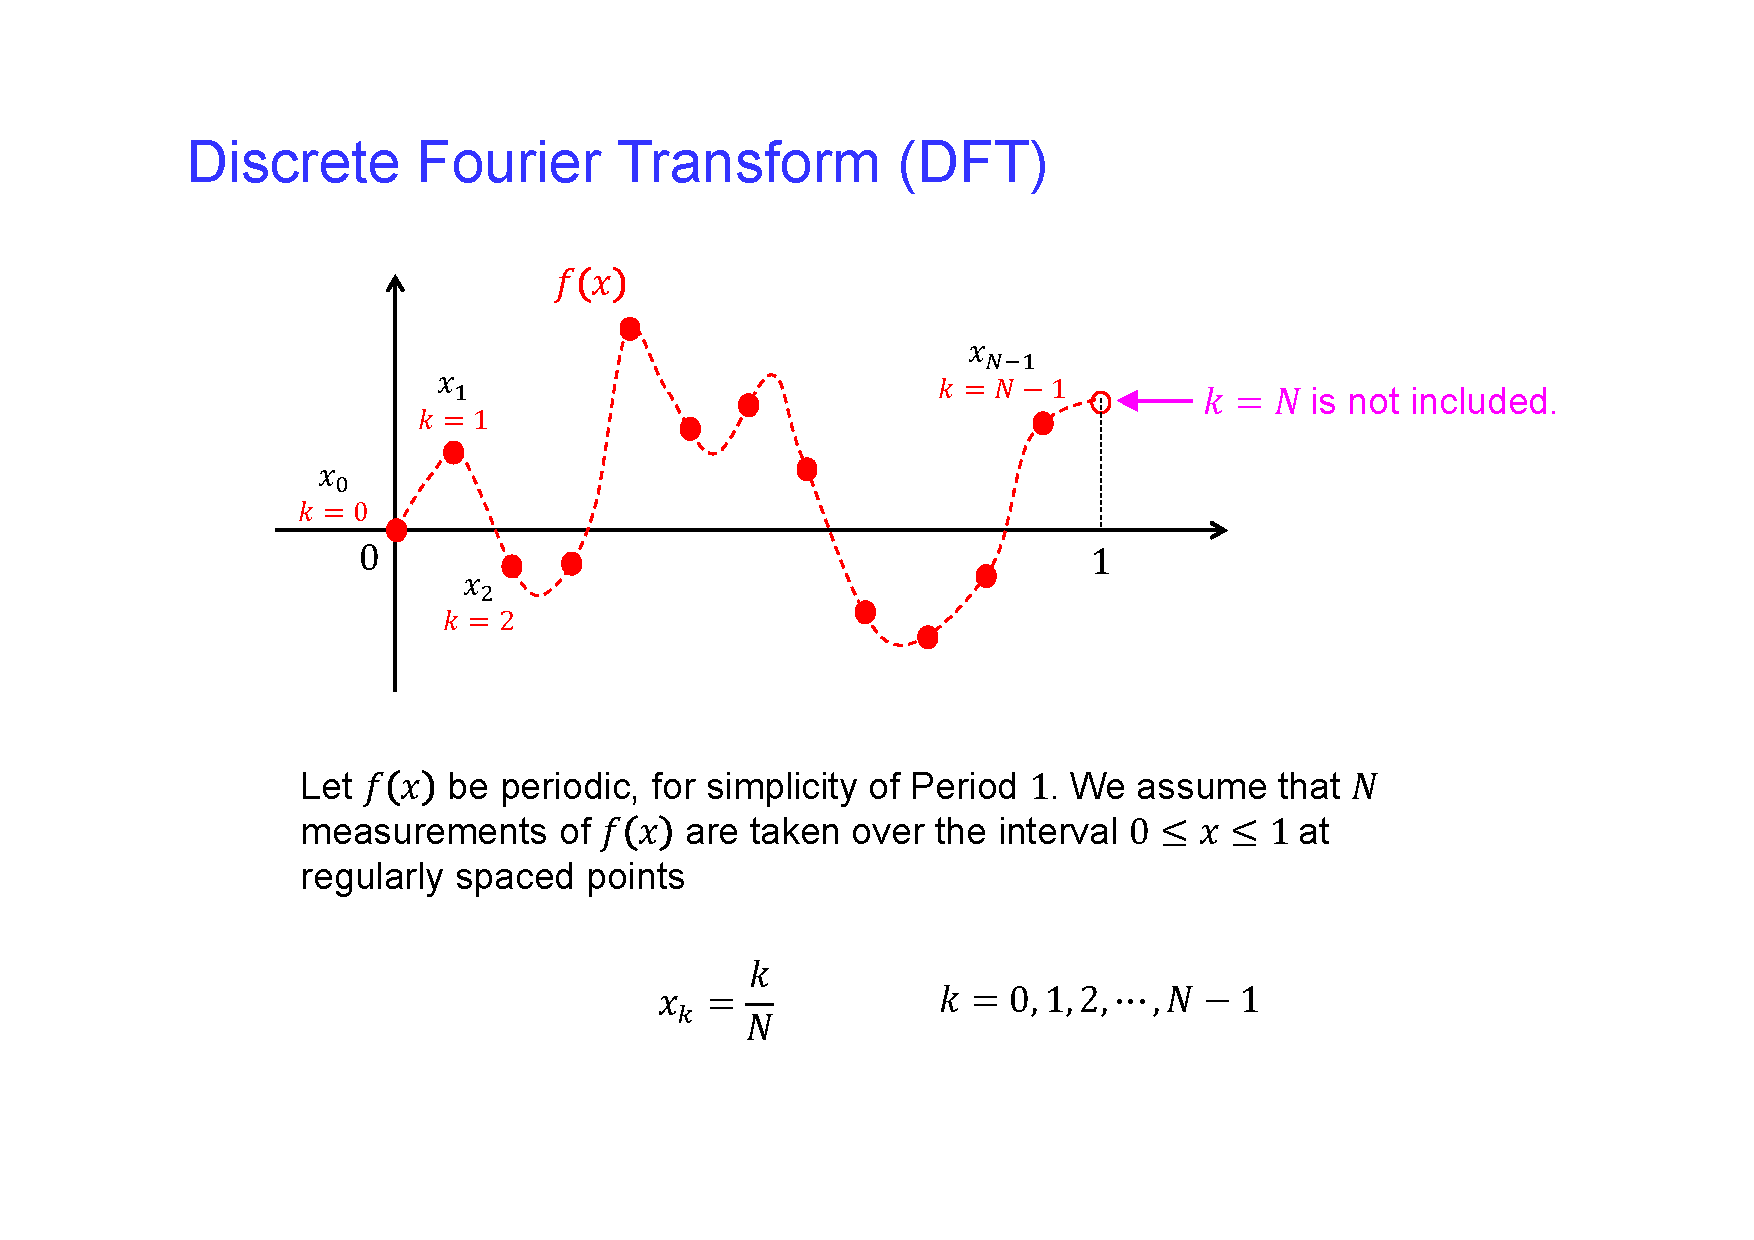
\includepdf[pages=-,pagecommand={},width=\textwidth,nup=1x2,frame=true]{discrete_10-15.pdf}

The challenge below considers sampling of a 1 Hz sine-wave 8 times per second, sampling at time 0, $\frac{1}{8}$, \ldots, $\frac{7}{8}$:

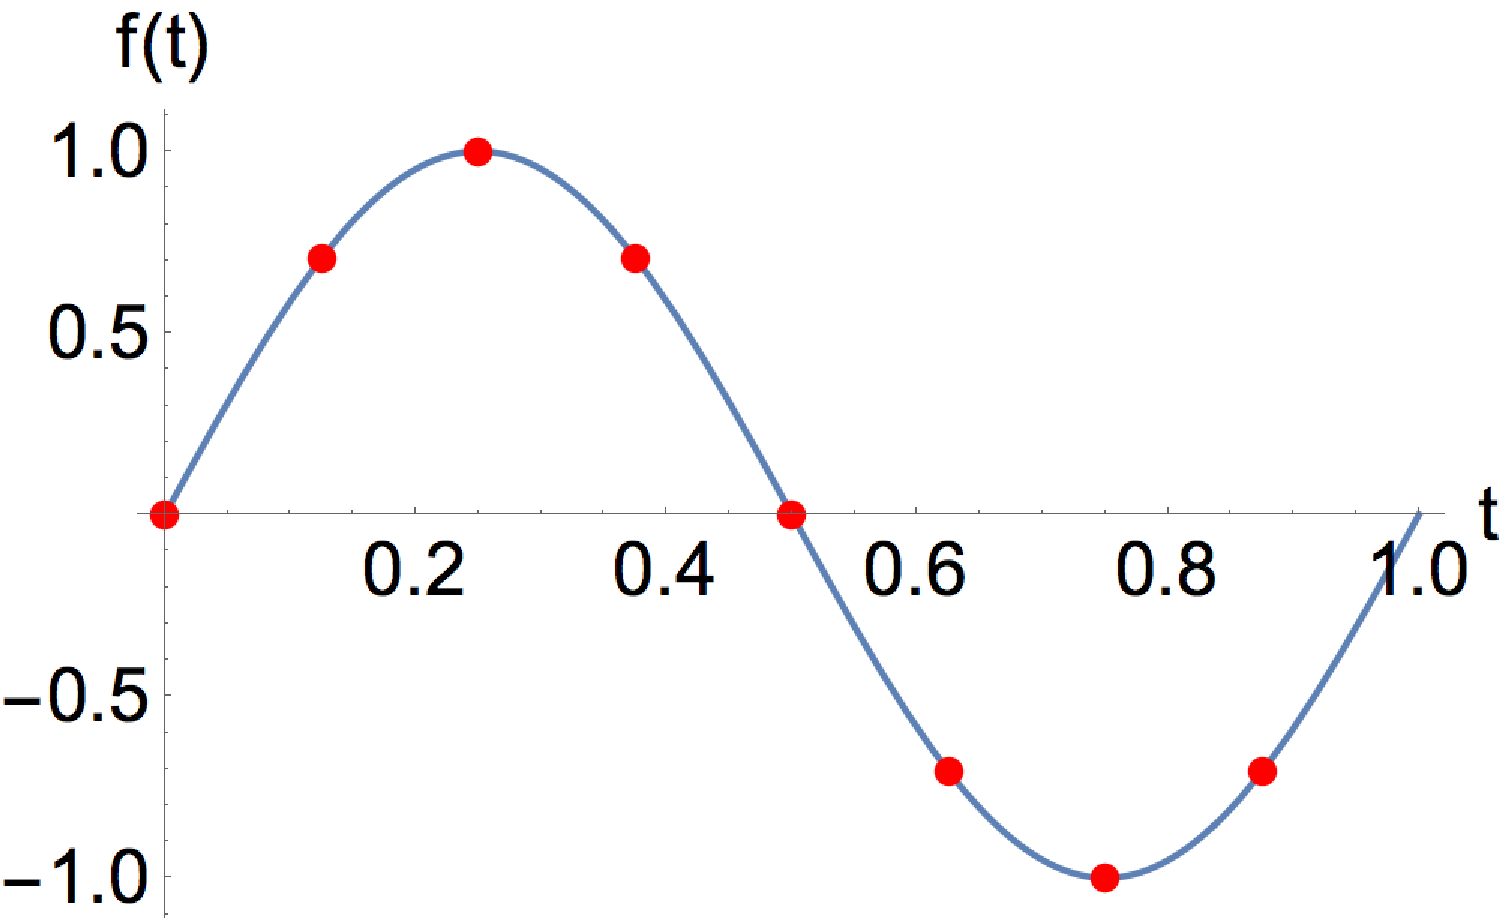
\includegraphics[scale=0.75]{sinedft.png}

This yields sample values of

\begin{equation}
f = \left(
\begin{array}{c}
 0 \\
 1/\sqrt{2} \\
 1 \\
 1/\sqrt{2} \\
 0 \\
 -1/\sqrt{2} \\
 -1 \\
 -1/\sqrt{2} \\
\end{array}
\right)
\end{equation}

\subsection*{Challenge}
Calculate the missing values A-H in the following calculation of the frequency spectrum:


\begin{equation}
    F_8 = 
    \left(
        \begin{array}{cccccccc}
             1 & \textbf{A} & \textbf{B} & 1 & 1 & 1 & 1 & 1 \\
             1 & \textbf{C} & \textbf{D} & -\frac{1+i}{\sqrt{2}} & -1 & -\frac{1-i}{\sqrt{2}} & i & \frac{1+i}{\sqrt{2}} \\
             1 & \textbf{E} & \textbf{F} & i & 1 & -i & -1 & i \\
             1 & -\frac{1+i}{\sqrt{2}} & i & -\frac{1-i}{\sqrt{2}} & -1 & \frac{1+i}{\sqrt{2}} & -i & -\frac{1-i}{\sqrt{2}} \\
             1 & -1 & 1 & -1 & 1 & -1 & 1 & -1 \\
             1 & -\frac{1-i}{\sqrt{2}} & -i & \frac{1+i}{\sqrt{2}} & -1 & -\frac{1-i}{\sqrt{2}} & i & -\frac{1+i}{\sqrt{2}} \\
             1 & i & -1 & -i & 1 & i & -1 & -i \\
             1 & \frac{1+i}{\sqrt{2}} & i & -\frac{1-i}{\sqrt{2}} & -1 & -\frac{1+i}{\sqrt{2}} & -i & -\frac{1-i}{\sqrt{2}} \\
        \end{array}
    \right) 
\end{equation}


\begin{equation}
    \hat{f} =
    \left(
        \begin{array}{c}
             \textbf{G} \\
             \textbf{H} \\
             0 \\
             0 \\
             0 \\
             0 \\
             0 \\
             4 i \\
        \end{array}
    \right)
\end{equation}

\subsection*{Solutions}

Enter imaginary numbers as shown in the table in section \ref{sec:hashes}. For example: $-1/\sqrt{2}-i/\sqrt{2}$ would be entered for \hash{abc}{a1b2c3} as ``abc\_re(-0.71)im(-0.71)'', $-i$ would be entered simply as ``abc\_im(-1.00)'' and $-1$ would just be ``abc\_-1.00''.

\begin{tabular}{|c|c|}
    \hline
    \textbf{A} & \hash{yyya}{b3a860} \\
    \textbf{B} & \hash{yyyb}{1058f4} \\
    \textbf{C} & \hash{yyyc}{e6bc8f} \\
    \textbf{D} & \hash{yyyd}{da2637} \\
    \textbf{E} & \hash{yyye}{696976} \\
    \textbf{F} & \hash{yyyf}{850784} \\
    \textbf{G} & \hash{yyyg}{dca1dd} \\
    \textbf{H} & \hash{yyyh}{cb48e5} \\
    \hline
\end{tabular}




%%%%%%%%%%%%%%%%%%%%%%%%%%%%%%%%%
\newpage
%%%%%%%%%%%%%%%%%%%%%%%%%%%%%%%%%
\section{Discrete Fourier Transform: Analysis}

\subsection*{Resources}
Having identified the frequency spectrum, it is possible then to analyse the frequencies of the signal. The video listed below provides a nice introduction into understanding our frequency spectrum. Note that it uses the ``j'' representation of imaginary numbers (instead of ``i'').

\begin{itemize}
    \item Video: \url{https://www.youtube.com/watch?v=mkGsMWi_j4Q}
\end{itemize}

\subsection*{Challenge}
What is the frequency, magnitude and phase of the sine-wave as determined through our discrete Fourier transform analysis?

\subsection*{Solutions}
Frequency: \hash{zzz}{874a2c}

Magnitude: \hash{aaaa}{2b946c}

Phase: \hash{bbbb}{132b51}




%%%%%%%%%%%%%%%%%%%%%%%%%%%%%%%%%
\newpage
%%%%%%%%%%%%%%%%%%%%%%%%%%%%%%%%%
\section{Analysing a more complex function: part I}

\subsection*{Challenge}
The following signal shown in the graph below has a fundamental frequency of 1 Hz:
\begin{equation}
    f(t) = Cos(2 \pi t) + Sin(4 \pi t)
\end{equation}

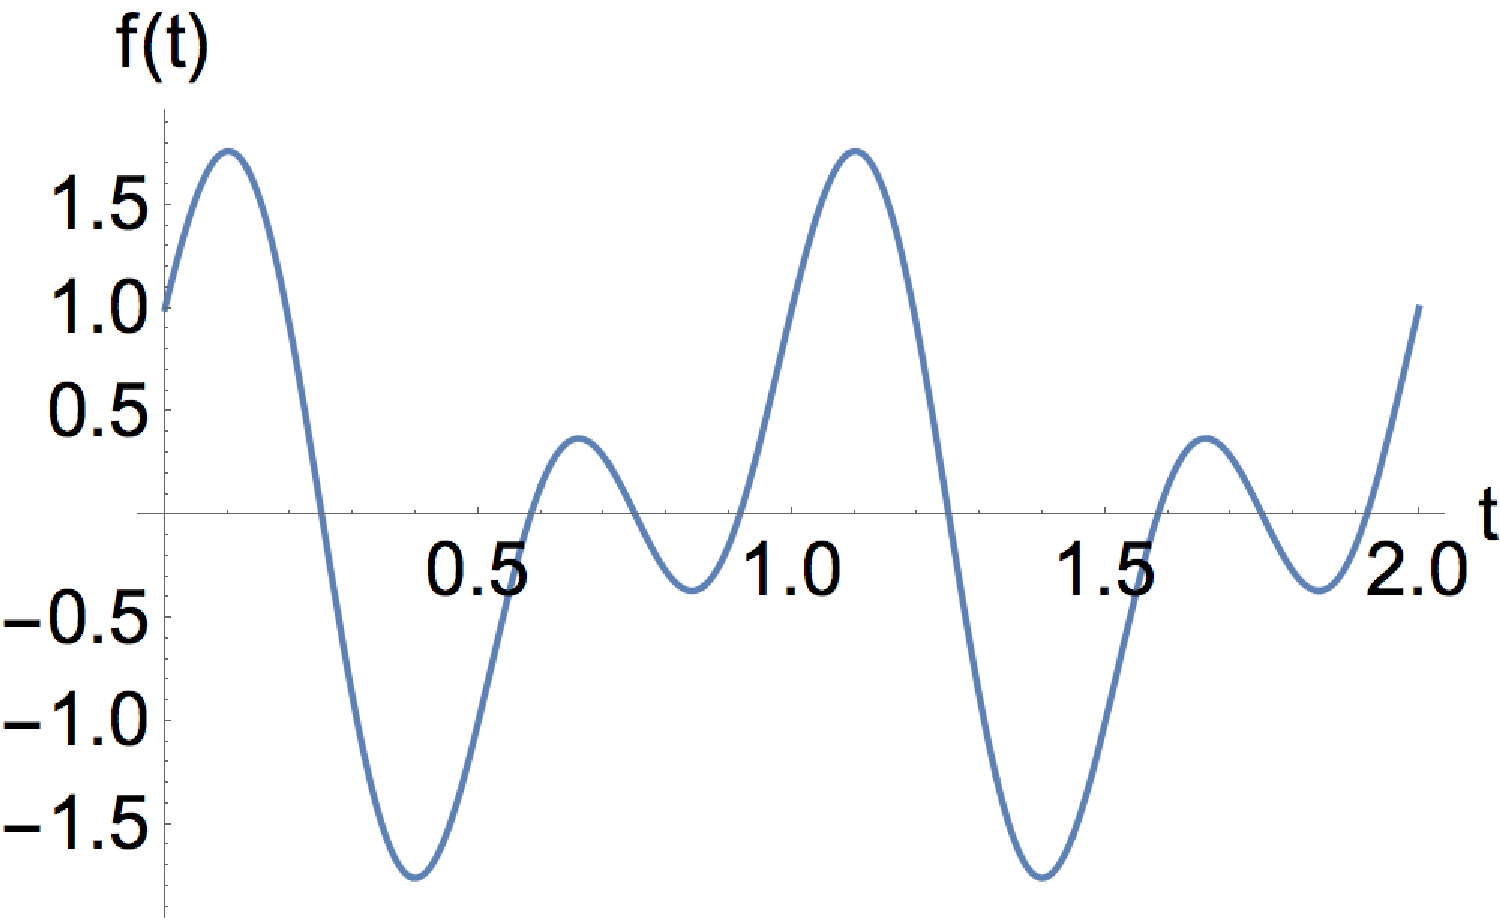
\includegraphics[scale=0.75]{dftcossin.png}

1. What are the two frequencies that make up the signal?

2. As described earlier, if you sample too infrequently, aliasing will occur. What is the maximum sampling frequency at which aliasing will occur for this signal?

\subsection*{Solutions}
1.\\
Lower frequency in Hz: \hash{cccc}{5a14e7}\\
Higher frequency in Hz: \hash{dddd}{1125b4}

2. \hash{eeee}{6ee287} times per second (or Hz)




%%%%%%%%%%%%%%%%%%%%%%%%%%%%%%%%%
\newpage
%%%%%%%%%%%%%%%%%%%%%%%%%%%%%%%%%
\section{Analysing a more complex function: part II}

\subsection*{Challenge}
Sampling the signal in the previous challenge 8 times per second:

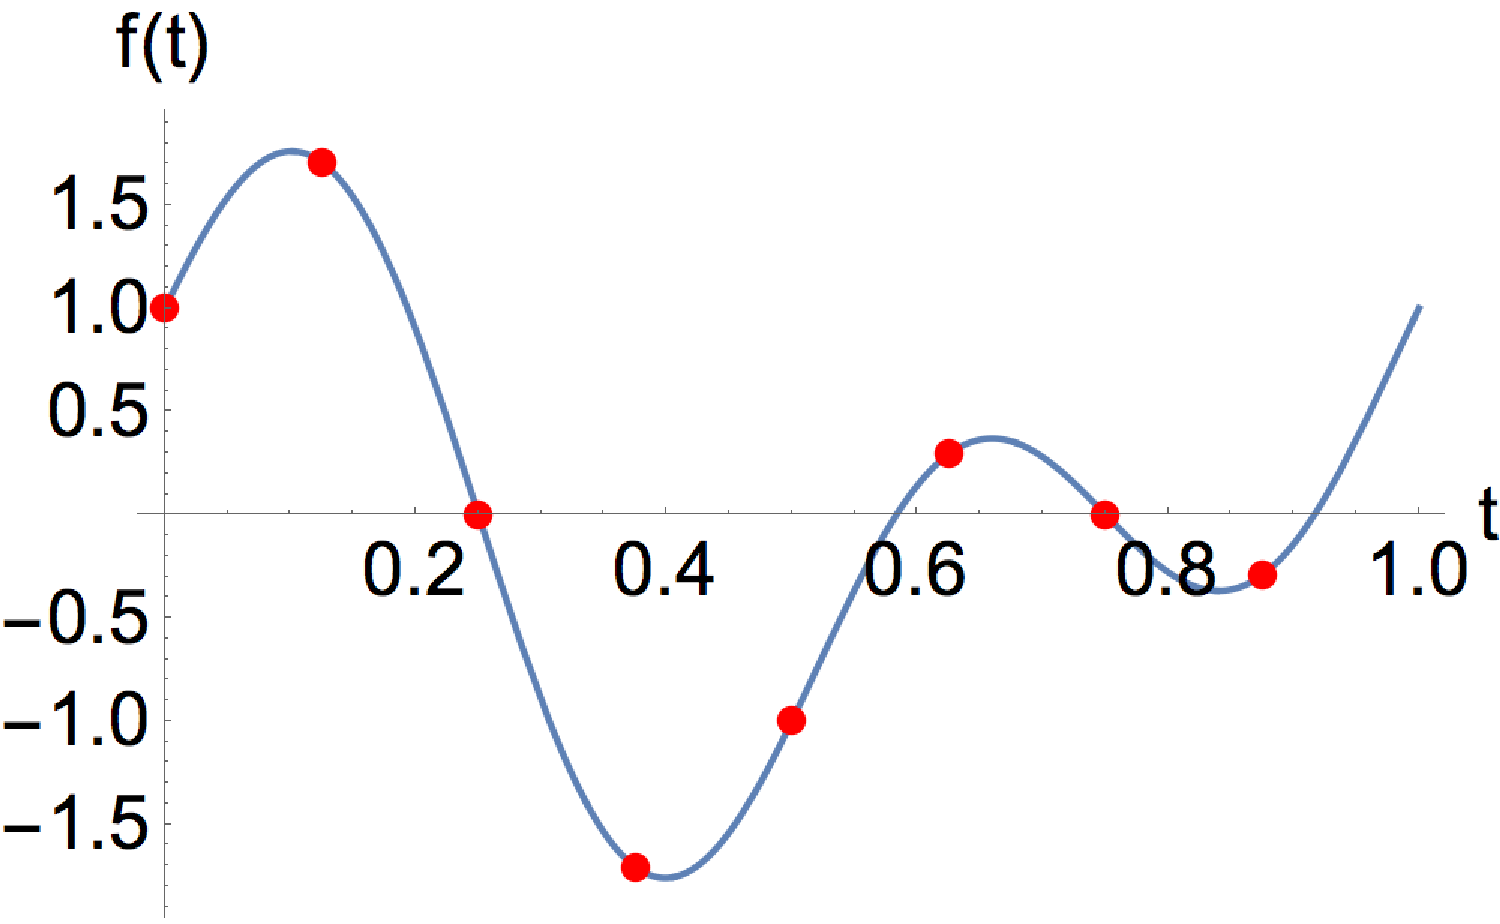
\includegraphics[scale=0.75]{dftcossinsamples.png}

yields values of
\begin{equation}
   \left(
\begin{array}{c}
 1. \\
 1.71 \\
 0. \\
 -1.71 \\
 -1. \\
 0.29 \\
 0. \\
 -0.29 \\
\end{array}
\right) 
\end{equation}

Calculating the matrix F yields

\begin{equation}
   \left(
\begin{array}{cccccccc}
 1 & 1              & 1 & 1 & 1 & 1 & 1 & 1 \\
 1 & (1-i)/\sqrt{2} & \bm{A} & -(1+i)/\sqrt{2} & -1 & (-1+i)/\sqrt{2} & i & (1+i)/\sqrt{2} \\
 1 & \bm{B}         & -1 & i & 1 & -i & -1 & i \\
 1 & -(1+i)/\sqrt{2}& i & (1-i)/\sqrt{2} & -1 & (1+i)/\sqrt{2} & -i & (-1+i)/\sqrt{2} \\
 1 & -1             & 1 & -1 & 1 & -1 & 1 & -1 \\
 1 & (-1+i)/\sqrt{2}& -i & (1+i)/\sqrt{2} & -1 & (1-i)/\sqrt{2} & i & -(1+i)/\sqrt{2} \\
 1 & i              & -1 & -i & 1 & i & -1 & -i \\
 1 & (1+i)/\sqrt{2} & i & (-1+i)/\sqrt{2} & -1 & -(1+i)/\sqrt{2} & -i & (1-i)/\sqrt{2} \\
\end{array}
\right) 
\end{equation}

1. Determine the missing values \textbf{A} and \textbf{B}.

2. Determine, by calculation, the frequencies with their magnitudes and phases of this signal. In this case, you can know the constituent frequencies, their magnitudes and phases because you know how the signal is made up of two signals. Check that your calculation aligns with your intuition.

\subsection*{Solutions}
1.\\
A = \hash{a}{d90da1}\\
B = \hash{b}{23ae42}

2. If you are not sure what your intuition should be, or if your answer does not match your intuition, please discuss with your partner or the teacher in class.


% NT: Go the other way to reconstruct a signal. Should spend an entire class on this.
